\documentclass{standalone}
\usepackage{tikz}

\begin{document}

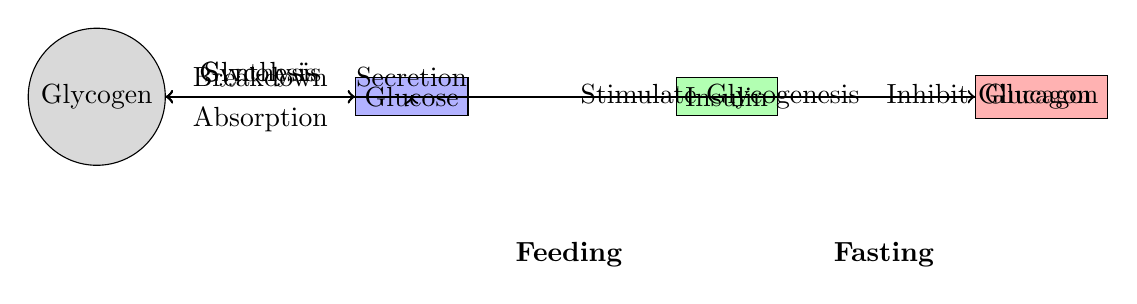
\begin{tikzpicture}[node distance=2cm]
    % Nodes
    \node (glycogen) [circle, draw, fill=gray!30] {Glycogen};
    \node (glucose) [rectangle, draw, fill=blue!30] at (4,0) {Glucose};
    \node (insulin) [rectangle, draw, fill=green!30] at (8,0) {Insulin};
    \node (glucagon) [rectangle, draw, fill=red!30] at (12,0) {Glucagon};

    % Feeding state
    \draw[->, thick] (glycogen) -- node[above] {Synthesis} (glucose);
    \draw[->, thick] (glucose) -- node[below] {Absorption} (glycogen);
    \draw[->, thick] (glucose) -- node[above] {Glycolysis} (glycogen);
    \draw[->, thick] (insulin) -- node[right] {Inhibit Glucagon} (glucagon);

    % Fasting state
    \draw[->, thick] (glycogen) -- node[above] {Breakdown} (glucose);
    \draw[->, thick] (glucagon) -- node[right] {Stimulate Glycogenesis} (glycogen);
    \draw[->, thick] (glucose) -- node[above] {Secretion} (glucose);

    % Labels
    \node at (6,-2) {\textbf{Feeding}};
    \node at (10,-2) {\textbf{Fasting}};
\end{tikzpicture}

\end{document}